%% 
%% Copyright 2007, 2008, 2009 Elsevier Ltd
%% 
%% This file is part of the 'Elsarticle Bundle'.
%% ---------------------------------------------
%% 
%% It may be distributed under the conditions of the LaTeX Project Public
%% License, either version 1.2 of this license or (at your option) any
%% later version.  The latest version of this license is in
%%    http://www.latex-project.org/lppl.txt
%% and version 1.2 or later is part of all distributions of LaTeX
%% version 1999/12/01 or later.
%% 
%% The list of all files belonging to the 'Elsarticle Bundle' is
%% given in the file `manifest.txt'.
%% 

%% Template article for Elsevier's document class `elsarticle'
%% with numbered style bibliographic references
%% SP 2008/03/01

\documentclass[preprint,12pt]{elsarticle}

%% Use the option review to obtain double line spacing
%% \documentclass[authoryear,preprint,review,12pt]{elsarticle}

%% Use the options 1p,twocolumn; 3p; 3p,twocolumn; 5p; or 5p,twocolumn
%% for a journal layout:
%% \documentclass[final,1p,times]{elsarticle}
%% \documentclass[final,1p,times,twocolumn]{elsarticle}
%% \documentclass[final,3p,times]{elsarticle}
%% \documentclass[final,3p,times,twocolumn]{elsarticle}
%% \documentclass[final,5p,times]{elsarticle}
%% \documentclass[final,5p,times,twocolumn]{elsarticle}

%% For including figures, graphicx.sty has been loaded in
%% elsarticle.cls. If you prefer to use the old commands
%% please give \usepackage{epsfig}

%% The amssymb package provides various useful mathematical symbols
\usepackage{amssymb}
\usepackage{booktabs}
\usepackage{amsmath}
\usepackage{algorithm}
\usepackage{lscape}
\usepackage[noend]{algpseudocode}
\usepackage{algcompatible}
\usepackage{multirow}


%% The amsthm package provides extended theorem environments
%% \usepackage{amsthm}

%% The lineno packages adds line numbers. Start line numbering with
%% \begin{linenumbers}, end it with \end{linenumbers}. Or switch it on
%% for the whole article with \linenumbers.
%% \usepackage{lineno}
\journal{Information Processing Letters}
\bibliographystyle{elsarticle-num}
\begin{document}

\begin{frontmatter}

%% Title, authors and addresses

%% use the tnoteref command within \title for footnotes;
%% use the tnotetext command for theassociated footnote;
%% use the fnref command within \author or \address for footnotes;
%% use the fntext command for theassociated footnote;
%% use the corref command within \author for corresponding author footnotes;
%% use the cortext command for theassociated footnote;
%% and the form \ead[url] for the home page:
%% \title{Title\tnoteref{label1}}
%% \tnotetext[label1]{}
%% \author{Name\corref{cor1}\fnref{label2}}
%% \ead{email address}
%% \ead[url]{home page}
%% \fntext[label2]{}
%% \cortext[cor1]{}
%% \address{Address\fnref{label3}}
%% \fntext[label3]{}

\title{Optimized and Cost Considering Huffman Code For Biological Data Transmission}

%% use optional labels to link authors explicitly to addresses:
%% \author[label1,label2]{}
%% \address[label1]{}
%% \address[label2]{}

\author{}

\address{}

\begin{abstract}
%% Text of abstract

\end{abstract}

\begin{keyword}
%% keywords here, in the form: keyword \sep keyword

%% PACS codes here, in the form: \PACS code \sep code

%% MSC codes here, in the form: \MSC code \sep code
%% or \MSC[2008] code \sep code (2000 is the default)

\end{keyword}

\end{frontmatter}

%% \linenumbers

%% main text
\section{Introduction}
\label{sec1}
In the recent years, application of battery-powered portable devices, e.g. laptop computers and mobile phones has increased significantly. Proper representation of digital data and their transmission efficiency has become a primary concern for digital community because it affects the performance, reliability, and the cost of computation in both portable and non-portable devices. CMOS technologies were developed in order to reduce the power consumption both in data processing and transmission. In order to increase transmission speed and reduce transmission cost, parallel data transmission methods are widely used. However, parallel transmission is limited to short distance communications, e.g. locally connected devices, internal buses. Ruling out the possible availability of parallel transmission links over long distance, we are left with its serial alternative only. If we attempt to transfer big files, e.g. DNA sequences, over a serial transmission link then it would take a significant amount of time. However, we cannot overlook this problem because at present parallel processing is widely used to increase throughput and in parallel processing architecture, processing units are usually distributed in different physical locations and task sharing is a must in such architecture.    

Data encoding techniques came into action to improve the data transmission efficiency over serial communication medium by compressing data before transmitting. Efficiency can be measured in terms of incurred cost, required storage space, consumed power, time spent and likewise. Data must be encoded to meet the purposes like: unambiguous retrieval of information, efficient storage, efficient transmission and etc. Let a message consist of sequences of characters taken from an alphabet $\Sigma$, where  $\alpha_1,\alpha_2,\alpha_3\ldots,\alpha_r$ are the elements that represent the characters in the source $\Sigma$. The length of $\alpha_i$ represents its cost or transmission time, i.e., $c\left(\alpha_i\right)= length(\alpha_i)$. A codeword $w_i$ is a string of characters in $\Sigma$, i.e., $w_i\in\Sigma^{+}$. If a codeword is $w_i=\alpha_{i1},\alpha_{i2},\ldots,\alpha_{in}$, then the length or cost of the codeword is the sum of the lengths of its constituent elements:

\begin{equation}
\label{eqn1}
  \text{cost}\left(w_i\right)=\sum_{j=1}^{n}c\left(\alpha_{ij}\right)
\end{equation} 
  
If all the elements of a codeword has unit cost or length then the cost of the codeword is equivalent to the length of the codeword. However, it is not necessary for the elements in the codeword to have equal length or cost. For example, in Morse Code all the ASCII characters are encoded as sequence of dots ($\cdot$) and dashes ($-$) where a dash is three times longer than a dot in duration \cite{Redmond09}. However, the Morse code scheme suffers from the prefix problem \cite{Gr03}. Ignoring the prefix problem, Morse code results in a tremendous savings of bits over ASCII representation. Using Morse code, we can treat the binary bits differently; 0 as a dot and 1 as a dash. Even if we consider the voltage level to represent the binary digits then they are still different. Table \ref{table1} shows the logic level to represent binary digits in CMOS and TTL technologies. 

\begin{table}[thpb]
\renewcommand{\arraystretch}{1.5}
\caption{Example of binary logic level}
\label{table1}
\centering
\begin{tabular}{c c c c}
\hline
 \bfseries Technology  & 0 & 1&Notes\\
\hline
\bfseries CMOS & $0~V$ to $\frac{V_{DD}}{2}$&$\frac{V_{DD}}{2}$ to $V_{DD}$&$V_{DD}$= supply voltage\\
%\hline
\bfseries TTL & $0~V$ to $0.8~V$&$2~V$ to $V_{CC}$ &$V_{CC}$ is $4.75~V$ to $5.25~V$\\
%\hline
\hline
\end{tabular}
\end{table}

As the unequal letter cost problem is not new therefore it has been addressed by different researchers. The more general case where the costs of the letters as well as the probabilities of the words are arbitrarily specified was treated in \cite{Karp61}. A number of other researchers have focused on uniform sources and developed algorithm for the unequal letter costs encoding \cite{Gil95, Kar62,Varn71,AltMel80,perl1975}.  Let $p_1,p_2,\ldots,p_n$ be the probabilities with which the source symbols occur in a message and the codewords representing the source symbols are $w_1,w_2,\ldots,w_n$ then the cost of the code $W$ is:

\begin{equation}
C\left(W\right)=\sum_{i=1}^{n}cost\left(w_i\right).p_i 
\end{equation}
The aim of producing an optimal code with unequal letter cost is to find a codeword $W$ that consists of $n$ prefix code letters each with minimum cost $c_i$ that produces the overall minimum cost $C\left(W\right)$, given that costs $0<c_1\leq c_2 \leq c_2 \ldots \leq c_n$, and probabilities $p_1\geq p_2\geq \ldots\geq p_n>0$.

Huffman code is an efficient data compression scheme that takes into account the probabilities at which different quantization levels are likely to occur and results in fewer data bits on the average. It is widely used to compress biological data, however, all the techniques use the classical form of the Huffman code where bits are treated equally. Out of many variations of the Huffman code where cost of bits are treated unequally, the most recent approach is described in \cite{Kab14}. This approach treated binary bit 0 as a dot $\left(\cdot\right)$ and 1 as a dash $\left(-\right)$ like Morse code and reduces the transmission cost (time) significantly. Like other variations of the cost considering Huffman code, the compression performance (in terms of number of bits require to encode a message) of this approach is not also better than classical Huffman code. In this paper, we have proposed a new optimised cost considering Huffman code based on the approach shown in \cite{Kab14}. This new approach optimised the number of bits require to encode a message while treating the binary bits unequally. The efficiency of the method is evaluated by applying it to compress some standard biological dataset.         

The rest of the paper is organised as follows: Section~\ref{sec2} presents the background study of the issues in biological data processing and the Huffman code. The proposed approach is described in Section~\ref{sec3}. Experimental results and discussion are presented in Section~\ref{sec4} . Finally, concluding remarks are presented in Section~\ref{sec5}.



\section{Background}
\label{sec2}
\subsection{Issues on Biological Data Transmission}
The size of biological data including DNA sequences increase with an ever expanding rate and will be bigger and bigger in the future. These Biological data are stored in biology database, the exponential growth of these database become a big problem to all biological data processing methods~\cite{Doug08}.
Different operation will be applied to these data such as, searching ~\cite{val10},e-mail attachment~\cite{chr09}, alignment ~\cite{che03}, and transmission on distributed computing ~\cite{cha14}. Interestingly, biological data compression can play a key role in all biological data processing.\\  
A recent deluge of interest in the development of new tools for biological data processing, these all algorithms needs an efficient methods for data compression. The main objective of data compression methods is minimizing the number of bits in the data representation. 
In ~\cite{bra09} authors propose a new general data structure and data encoding approach for the efficient storage of genomic data. This method encode only the differences between a genome sequence and a reference sequence, the method use different encoding scheme from fixed codes such as Golomb, Elias codes and variable codes such as Huffman codes. Other methods based on same idea to encode only the difference between reference sequence and the target one, Authors in \cite{chr09} uses Huffman code for encoding difference between sequence to sent it as an email attachment, but these methods suffer that they must sent the reference sequence for at least one time for each species.\\
Wang and Zhang \cite{wan11} proposed a new scheme for referential compression of genomes based on the chromosome level. The Algorithm aim to search for longest common subsequence between matching parts and the differences encoded using Huffman coding.\\
All previous studies focus only on the differences and the relation between continuation of the sequence, and without improvement of the encoding scheme.

%\subsection{Rationale of Unequal Bit Cost Considering Encoding Approaches}


\subsection{Huffman Codes}
In computer science and information theory, Huffman code is an entropy encoding algorithm used for lossless data compression. It takes into account the probabilities at which different symbols are likely to occur and results into fewer data bits on the average. 
%then assigns variable-length codes to different distinct symbols, and thus minimises the number of bits required to encode a message. 
For any given set of symbols and associated occurrence probabilities, there is an optimal encoding rule that minimises the number of bits needed to represent the source. Encoding symbols in predefined fixed length code, does not attain an optimum performance, because every character consumes equal number of bits irrespective to their degree of contribution to the whole message. Huffman code tackles this by generating variable length codes, given a probability usage frequency for a set of symbols. It generates prefix-code to facilitate unambiguous retrieval of information. A scheme of prefix code assigns codes to letters in $\Sigma$ to form codeword $w_i$ such that none of them is a prefix to another. For example, the codes $\left\{ 1,01,001,0001\right\}$ and $\left\{ 000,001,011,111\right\}$ are prefix-free, whereas the code $\left\{ 1,01,100\right\}$ is not, because 1 is a prefix in 100.

Applications of Huffman code are pervasive throughout
computer science. The algorithm to completely perform Huffman encoding and decoding is explained by \cite{Amst86}. It can be used effectively where there is a need for a compact code to represent a long series of a relatively small number of distinct bytes. For example, Table \ref{table1} shows 8 different ASCII characters, their frequencies, ASCII codes and the codewords generated for those symbols using Huffman code. It is seen from the table that the codeword to represent each character is compressed and the most frequent character gets the shortest code. In this example, the compression ratio obtained by Huffman code is 64.16\%.   

\begin{table}[thpb]
\renewcommand{\arraystretch}{1.3}
\caption{Example of application of Huffman Code to compress ASCII characters}
\label{table2}
\centering
\begin{tabular}{c c c c}
\hline
 Symbols & Frequency& ASCII Code &\begin{tabular}{@{}c@{}}Codewords using\\Huffman Code\end{tabular} \\
\hline
\bfseries A & 50&01000001&00\\
%\hline
\bfseries B & 35&01000010&101\\
%\hline
\bfseries C & 42&01000011&110\\
%\hline
\bfseries D & 22&01000100&1001\\
%\hline
\bfseries E & 65&01000101&01\\
%\hline
\bfseries F & 25&01000110&1111\\
%\hline
\bfseries G & 9&01000111&1000\\
%\hline
\bfseries H & 23&01001000&1110\\
\hline
\end{tabular}
\end{table}

There are many other variants of Huffman codes that compress source data to reduce data size and/or transmission cost. For example, Mannan and Kaykobad introduced block technique in Huffman coding which overcomes the limitation of reading whole message prior to encoding\cite{Kay03}. In classical Huffman coding scheme, the letter costs are considered as equal. The unequal letter cost versions of Huffman codes scheme are proposed in \cite{Gol1996,Gol02,Gol2002,Gol12}.
In the unequal letter cost version of the classical Huffman code, letters  of  the alphabet  are  considered as unequal. Recently, in \cite{Kab14} a method is proposed to show the effects of unequal bits cost on classical Huffman code. The idea of this method is to assign the most frequent symbol the minimum cost and the least frequent symbol the maximum cost code, whereas classical Huffman code assigns most frequent symbol the minimum length and the least frequent symbol the maximum length code.

\section{Approach}
\label{sec3}
\subsection{Proposed Scheme}

A genome is a stretch of DNA (or RNA) that codes for a polypeptide (protein), that is a set of amino acids bound together in specific order. Each genomic sequence consist of nucleotide bound together, which are interpreted by the cellular machinery in groups of three, called triplets~\cite{}. This is the main raison to divide the whole sequence in a set of triplet and give a code to each triplet. The first step in the optimised cost considering algorithm is cutting the sequence in triplet, then compute the frequency of each triplet in the whole sequence. This table of frequencies are used by the cost considering Huffman code to generate low cost code to each triplet (frequency). Finally these codes with frequencies are used by the optimised cost considering algorithm to generate the optimal allocation with a given  penalty.

\begin{figure}[thpb]
\begin{center}
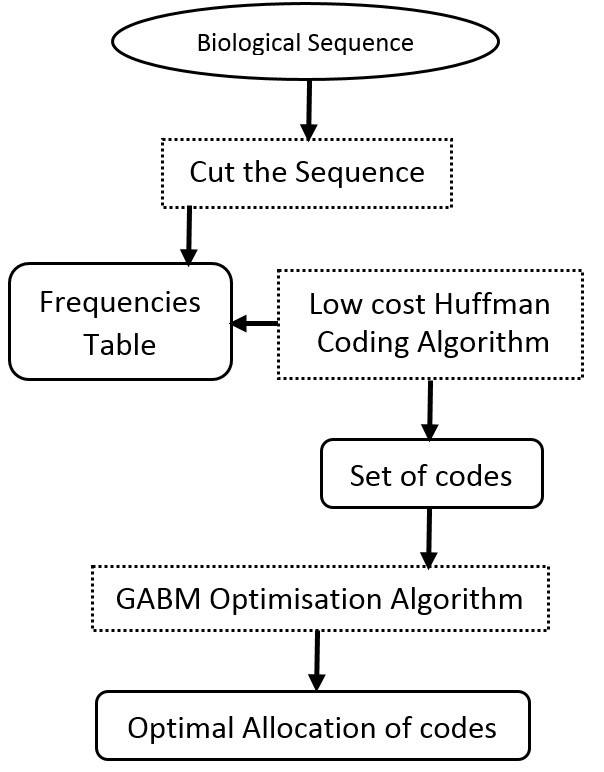
\includegraphics[scale=0.5]{Images/Drawing3.jpg}
\caption{The proposed Scheme}
\end{center}
\label{Fig1}
\end{figure}

\subsection{Cost Considering Huffman code}
The classical Huffman algorithm aims at reducing total number of bits and it constructs the tree in a bottom up fashion. It is shown in \cite{golin98} that if the costs of letters are considered unequal then the straightforward bottom up greedy approach does not work. Authors in \cite{Kab14} uses a top down approach to build a binary tree considering unequal letter cost of bits. They considered cost (length) of 0 and 1 as integer constants $\alpha$ and $\beta$, and  $\alpha < \beta$. The complete algorithm to obtain an optimal prefix-free code for unequal letter cost is shown below. The input to the algorithm are the distinct symbols contained in the message to be encoded and their frequencies. The process of creating the binary tree starts with a single node (root node) and it is initialised with cost 0.  After that, two child (leaf) nodes are created for the root node, i.e. level of the tree is increased by one. Cost of the left child is calculated as the summation of the cost of its parent node and the length of the left arc, and cost of the right child is calculated as the summation of the cost of its parent node and the length of the right arc. Length of left and right arcs are actually the cost (length) of 0 ($\alpha$) and 1 ($\beta$) respectively. The next step is to take a child node with least cost and create two child nodes for it and make it a parent node. In this way, in every iteration the child node with least cost becomes a parent node with two new child nodes. Creation of new child nodes is stopped when total number of child nodes become equal to the number of distinct symbols needed to be encoded. 

Now the tree $T$ is constructed and the cost of the tree actually depends on how we assign the frequencies to the leaf nodes. The overall cost will be minimised if the leaves with highest cost always have smaller or equal weight (frequency). To fulfil this condition the leaves of the $T$ are enumerated in non-decreasing order of their cost, i.e., $cost(l_1)\leq cost(l_2)\leq \ldots \leq cost(l_n),$ and that $f_1 \geq f_2 \geq \ldots\geq f_n$, where $l_i$ and $f_i$ are leaf node and frequency of distinct symbol respectively $for~ i=1,2,\ldots n$ . The frequency or weight of parent nodes are calculated as the sum of its child nodes, and it continues upwards until the root node is reached. After that, the algorithm checks for any possible conflicts between all pair of nodes. Two nodes are considered as conflicted if the node with higher cost has higher frequency violating the above condition, i.e., if $cost(l_i)> cost(l_j)~and~f(l_i)>f(l_j)$, then there remains a conflict.  If there remains a conflict between nodes, then it is resolved by swapping the nodes and recalculating the cost of the tree downward and frequency of the nodes upward.  When all the conflicts if existed are resolved then the algorithm generates codes for each of the distinct symbols.   
\begin{algorithm}[!btph]
\caption{Cost-considering / Unequal bit cost Coding}
\label{alg1}

\begin{algorithmic}[1]
\REQUIRE Distinct symbols contained in the message to be encoded and their frequencies 
\ENSURE Non-uniform\ /\ variable\ letter\ cost\ i.e,\ Cost-considering\ balanced\ tree

\FOR{each distinct symbol $i$} 
\STATE $ Enqueue\left(max\_Q , frequency~[~i~]\right)$
\ENDFOR
\STATE create a root node
\STATE $cost~[~root~]\leftarrow 0$
\STATE $Enqueue\left(min\_Q , cost~[~root~]\right)$
\STATE Define costs of the left and right child of the binary tree
\REPEAT 
\STATE $cost\_of\_parent\_node\leftarrow Dequeue\left(min\_Q\right)$
\STATE create $left$ and $right$ child for this node
\STATE $cost~[~left\_child~]\leftarrow cost\_of\_parent\_node+left\_child\_cost$
\STATE $Enqueue\left(min\_Q , cost~[~left\_child~]\right)$
\STATE $cost~[~right\_child~]\leftarrow cost\_of\_parent\_node+right\_child\_cost$
\STATE $Enqueue\left(min\_Q , cost~[~right\_child~]\right)$
\STATE Mark parent node as explored
\UNTIL{$2\left(n-1\right)$ nodes are created}
\WHILE{$min\_Q\neq\emptyset$} 
\STATE $leaf\_node\leftarrow Dequeue\left(min\_Q\right)$
\STATE $frequency[leaf\_node]\leftarrow Dequeue\left(max\_Q\right)$
\ENDWHILE
\FOR{each parent node $j$} 
\STATE $frequency~[~j~]\leftarrow frequency~[~left\_child~]+frequency~[~right\_child~]$
\ENDFOR
\REPEAT
\IF{conflict between nodes} 
\STATE resolve conflict by swapping conflicted nodes
\STATE calculate and reassign cost of all affected nodes
\STATE calculate and reassign frequency of all affected nodes 
\ENDIF
\UNTIL{all conflicts are resolved }
%\algstore{myalg}
\end{algorithmic}
\end{algorithm}
\subsection{Optimisation of the Codes}
\subsubsection{Problem formulation}
The problem of finding the best allocation of codes to each symbol can be   modelled as an Assignment Problems with Constraint, the problem is formulated as follows :\\\\
\textbf{Definition:} Given a set of codes $C=\left\{C_{1},C_{2}...C_{n}\right\}$, and a set of frequencies $C=\left\{Q_{1},Q_{2}...Q_{n}\right\}$. For each code we have the length of the code $|C_{i}|$ (number of bits) and the cost of the code $S_{C_{i}}$ (cost of ones and zeros), the objective is to assign to each frequency a code in order to minimize the total number of bits, while respecting the initial assignment total cost $S_{t}$ with a given penalty $\lambda$. This penalty coefficient represent the allowed Marge can be sacrificed for cost to optimize number of bits    
\\
The Objective Function is : 

\begin{equation}
Minimise \sum (|C_{i}| \times Q_{j}) 
\end{equation}
while :
\begin{equation}
\sum (|S_{C_{i}}| \times Q_{j}) \leqslant (\lambda+1) S_{t} 
\end{equation}

\subsubsection{Basic Genetic Algorithm}
Genetic Algorithm (GA) is a bio-inspired meta-heuristics algorithm developed by []. GA is a stochastic optimization algorithm imitate the natural evolution process of genomes. GA started by generate a population of random feasible solutions, the optimization process of GA is as follow, and we select two solution among the population, by one of the well-known selection techniques. This two selected solution will be considered as two parents, we generate two other new solutions from the two selected solution (Sons), this new solutions can be mutate according to a given mutation probability. The quality of each solution is computed with the fitness function which control the evolution of the GA population by the deletion of the worst solution and insertion of the good solutions among   parents and sons. This processes is repeated until the stopped criteria is achieved which can be the number of generation or if the population is stabilized.
\subsubsection{GA for Bits minimisation}
The main objective of the GA optimisation algorithm for bits minimisation (GaBm) problem is to assign to each frequency a specific code. The encoding of an optimization problem solution into a
chromosome is one of the most important issue to obtaining a good optimisation results. GaBM uses a two array fixed length to "64" which is the number of combination for all nucleotides, the first contain the frequencies of each codes and the second contain the cost of each codes. In this way, our genetic algorithm will work with the two array and uses the entry index on the allocation process.
The genetic algorithm are stochastic algorithm based on random evolution. Generally the initial population is generated in a random affectation. In the GaBm algorithm the population contain firstly the affectation given by the cost considering Huffman code algorithm and secondly the rest of the population is random generated, but all generated solution must satisfy the initial cost constraints (step 1). 

The evolution of the population is the key of the optimisation algorithm of genetic algorithm. During each generation the process start with the selection of a proportion of the population to bread a new generation. In the literature many selection methods have been proposed to guide the population evolution. The existent selection methods are varied from a random selection to heuristic based selection. we have chosen to select randomly the part of the population to be processed, as the heuristic methods are very time-consuming (step 3).
After that the operations of genetic algorithms are applied for the initial population to generate a new generation of the population (see figure 3). Firstly the crossover operation are applied to these two selected solution (considered as parents) to generate two new solutions (considered as sons)(step 4). In the literature many crossover techniques have been used in genetic algorithm, such as one-point crossover which divide the chromosome on two fragments and recombine the second fragments by the other chromosome second fragment, two-point crossover which divide the chromosome on three fragment and recombine the middle fragment by  the middle fragments on the other chromosome, and many other crossover techniques to allow a good convergence of the algorithm, in our case we have used the two point crossover with two parameters, the first parameter $\alpha$ is a random value in [0,63], which represent the first cut point and $\beta$ is a random value too in [0,63], which represent the number of position to be crossed. we used a two random parameters to ensure a good diversification on the whole search space (step 4).
These two new generated children may contain conflict like finding a duplicated code allocated to two different frequencies in the solution, so a regulation step is done to ensure the correctness of the solution (see figure 3).
 Secondly these two new solutions are mutated according to a predefined probability $\gamma$, the best value of mutation rate is very problem specific (step 5). The probability $\gamma$ are fixed to $0.2$ to explorer a few position on the solution. The mutation operator used to maintain genetic diversity from one generation of a population of genetic algorithm chromosomes to the next. In our case we have used the mutation as a random swap mutation operator (see figure 3).  Each new generated solution must satisfy the cost constraint, these children must be valid with satisfying the cost constraint. The next step is to add these two new solutions (children) to the population (step 7) (see figure 2). Finally the new population are ranked by fitness (step 8), and the worst solution are deleted until the initial size of the population are achieved  (step 9). the whole process are repeated until the max number of operation is achieved (step 10). 
\begin{algorithm}
\caption{GA for bits minimisation}
\begin{algorithmic}[1]
\State Population initialization (P).
\While {Max number of generation not achieved} 
\State Select two solutions $S_{1},S_{2}$ form P.
\State Crossover $S_{1},S_{2}$ to generate $S_{11},S_{21}$ (Children).
\State Mutate $S_{11},S_{21}$.
\State Validate children with cost constraint (equation 4). 
\State Add children to population
\State Rank the population by fitness
\State Remove worst candidates until population limit
\State Return to 2;
\EndWhile
\State Display the best solution from the population P;
\end{algorithmic}
\end{algorithm}

\begin{figure}[h]
\begin{center}
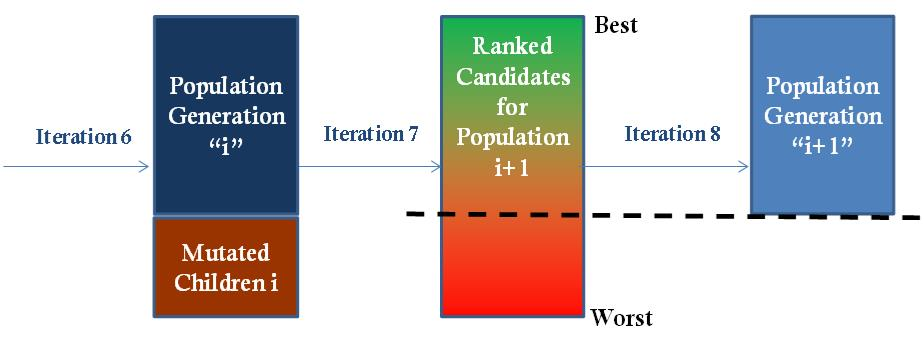
\includegraphics[scale=0.7]{Images/Drawing1.jpg}
\caption{Population Update for genetic algorithm}
\end{center}
\label{Fig2}
\end{figure}
\begin{figure}[h]
\begin{center}
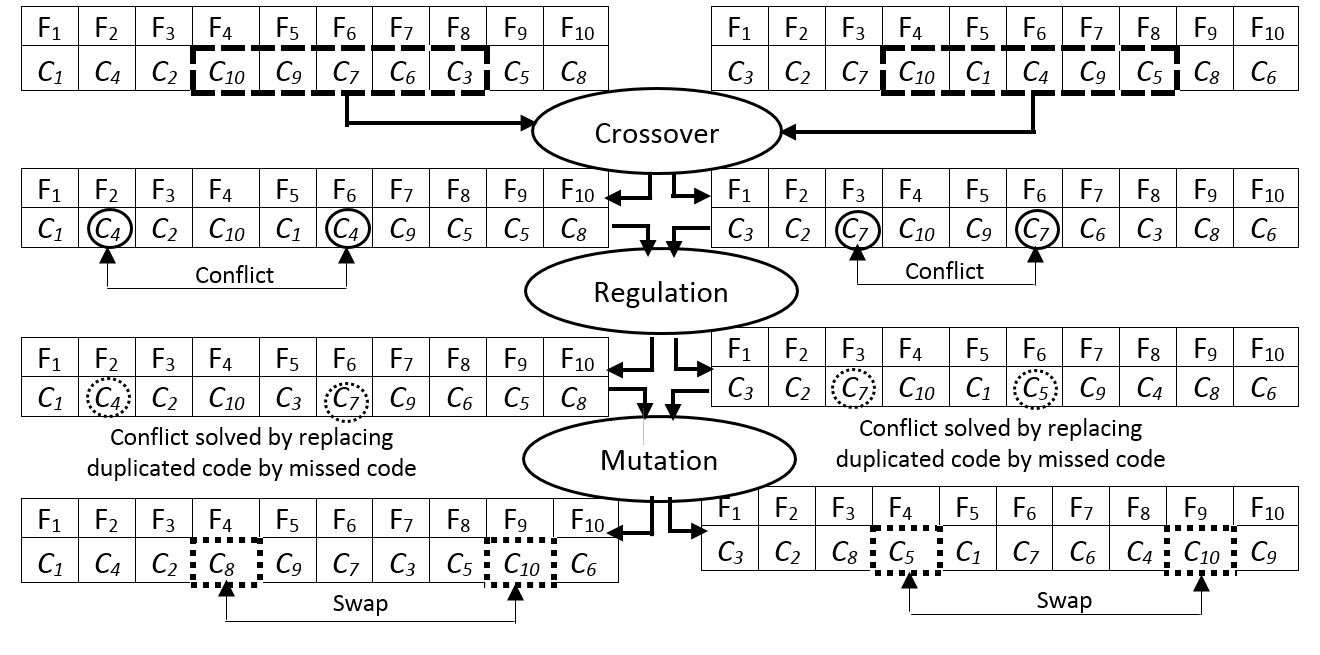
\includegraphics[scale=0.5]{Images/Drawing2.jpg}
\caption{Operations of genetic algorithm}
\end{center}
\label{Fig3}
\end{figure}



\section{Results And Discussion}
\label{sec4}
The approach has been evaluated with different real biological data (genomes), these genomes from The National Center for Biotechnology Information (NCBI) available on ( http://www.ncbi.nlm.nih.gov) []. In table () the different data set are described with the size of each of them and the references on the biological data bank.
\begin{table}
\small
\label{datas}
\caption{Dataset description}
\begin{center}
\begin{tabular}{c  c  c c}
\toprule
$\textbf{Data sets}$ &$\textbf{Name}$ &	$\textbf{Size (bp)}$ &	$\textbf{Reference}$ \\\hline
Genome 1& Mycobacterium smegmatis &6,988,302 & CP009496  \\\hline

Genome 2& Amycolatopsis benzoatilytica &  8,704,271& NZ\_KB912942 \\\hline

\multirow{2}{*}{Genome 3}&Mycobacterium rhodesiae& \multirow{2}{*}{6,415,739} & \multirow{2} {*}{CP003169}\\ 
&NBB3& &\\
\hline

\multirow{2}{*}{Genome 4 }&Streptomyces bottropensis& \multirow{2}{*}{8,955,726} &
\multirow{2}{*}{NZ\_KB911581} \\ 
& ATCC 25435 \\
\hline
    
\multirow{2}{*}{Genome 5}&Mycobacterium smegmatis& \multirow{2}{*}{6,988,269 } &\multirow{2}{*}{CP009494             } \\ 
&str. MC2 155 \\
\hline

\multirow{2}{*}{Genome 6}&Mycobacterium smegmatis& \multirow{2}{*}{7,092,137} &\multirow{2}{*}{NZ\_KI421511}\\   &MKD8& &\\
\hline
    
Genome 7& Bradyrhizobium WSM471& 7,784,016  &NZ\_CM001442\\\hline

\multirow{2}{*}{Genome 8}&Amycolatopsis thermoflava&  \multirow{2}{*}{8,677,910} &\multirow{2}{*}{NZ\_CM001442}\\   &N1165 & \\
\hline

\multirow{2}{*}{Genome 9}&Bacillus thuringiensis&   \multirow{2}{*}{6,026,843} &\multirow{2}{*}{ NZ\_CM000747 }\\    &Bt407&\\
\hline    

\multirow{2}{*}{Genome 10}&Bacillus thuringiensis& \multirow{2}{*}{6,323,123 } &\multirow{2}{*}{ NZ\_CM000748}\\    &serovar thuringiensis& \\
\hline
    
\multirow{2}{*}{Genome 11}&Pseudomonas aeruginosa& \multirow{2}{*}{6,801,503  } &\multirow{2}{*}{NZ\_AFXI01000001}\\    &9BR&\\
\hline
    
\multirow{2}{*}{Genome 12}&Bacillus thuringiensis&  \multirow{2}{*}{6,260,142  } &\multirow{2}{*}{ NZ\_CM000753}\\    &serovar berliner ATCC &\\
\hline
    
\multirow{2}{*}{Genome 13}&Bacillus thuringiensis& \multirow{2}{*}{6,037,513 } &\multirow{2}{*}{ NZ\_CM000750 }\\    &serovar pakistani&\\
\hline
    
\multirow{2}{*}{Genome 14}&Pseudomonas aeruginosa& \multirow{2}{*}{6,591,121  } &\multirow{2}{*}{ CP006982  }\\    &LES400&\\
\hline
\bottomrule
\end{tabular}
\end{center}
\end{table} 
The table 3 present the results founded by the basic Huffman code, cost considering algorithm and optimised cost considering algorithm. The result show that the number of bits of Huffman algorithm is the minimum number among the other algorithm but the cost is  very high. The cost considering algorithm improve the quality of the generated codes in terms of cost but the number of bits. The optimised cost considering algorithm try to find the best allocation of codes to frequencies while the cost constraint respected. The table 4 present the best founded number of bits with different penalty, for each genome we find the max number of useful penalty, after this value, increasing the penalty are in-useful (See figure 3), the number of bits achieve the minimum number but the cost stop decreasing (point 1 in figure 3) and this number of bits stabilized while the cost still increasing until it stabilized also (point 2 figure 3), after this point the cost and number of bits are stabilized.
\begin{table}
\small
\label{datas}
\caption{GABM for comparison for cost and number of bits of different approaches with different datasets}
\begin{center}
\begin{tabular}{c | c c | c c | c c}
\toprule
$\textbf{Data sets}$ & \multicolumn{2}{c}{Huffman Algorithm} & \multicolumn{2}{c}{CCA }& \multicolumn{2}{c}{OCCA}\\\hline
 & $\textbf{Cost}$	& $\textbf{Bits}$ &	$\textbf{Cost}$&	$\textbf{Bits	}$&$\textbf{Cost}$&	$\textbf{Bits}$
\\\hline
Genome 1&76787151  &	37256819	&67416213 & 41332479	& 67416213 & 40503061 \\\hline
Genome 2& 100425402 &  	48778740	& 88430665	& 54662727	& 88430665&  53341739 \\\hline
Genome 3&75940155  	&36860555	&66745619	&40927187 &	66745619 & 40182241\\\hline
Genome 4&103552729  	&50047265	&90821835&	56147481&	90821835  & 54319891\\\hline
Genome 5&82234926  &	39772838	&71963876	&44254676 &	71963876 & 43392820\\\hline
Genome 6&83454842  	&40370894	&73038795	&44864009	&73038795 & 44003571\\\hline
Genome 7&92539488  &	44977876&	81416359&	49790957	&81416359 & 49127335\\\hline
Genome 8&99613856 & 	48183688	&87102639&	53817307	&87102639&	52858893\\\hline
Genome 9&71876739 &	34874617&	62998800 &	38469200&	62998800 8&	37831964\\\hline
Genome 10&75324432 & 	36576034	&66084958&	40409906	&66084958&	39739522\\\hline
Genome 11&80766360  &	39092450&	70620666	&43119140&	70620666&	42359156 \\\hline
Genome 12&74560825  &	36179579&	65359604	&39926210	&65359604&	39221148\\\hline
Genome 13&71562941 & 	34737083	&62758225 &	38299629&	62758225 &	37809443\\\hline
Genome 14&78261299 & 	37843793&	68354090&	41816580&	68354090&	 41050420\\\hline
\bottomrule
\end{tabular}
\end{center}
\end{table}

\begin{table}
\small
\label{datas}
\caption{influence of penalty on bit minimization}
\begin{center}
\begin{tabular}{c c c c }
\toprule
$\textbf{Data sets}$ & $\textbf{Cost}$	& $\textbf{Bits}$ &		\textbf{$\lambda (\%)$} \\\hline
Mycobacterium smegmatis &	 70760174 &37809636& 4\\\hline
Amycolatopsis benzoatilytica &	92010490& 49654132& 3\\\hline
Mycobacterium rhodesiae&	69421783& 37563017 &3\\\hline
Streptomyces bottropensis&	96294638& 50330594& 5\\\hline
Mycobacterium smegmatis. MC2&	74855668 &40380464& 5\\\hline
Mycobacterium smegmatis MKD8&	76738330& 40782100 &4\\\hline
Bradyrhizobium WSM471&	84667949 &45961149& 3\\\hline
Amycolatopsis thermoflava&	92416243 &48336727& 5\\\hline
Bacillus thuringiensis serovar thuringiensis&	66145783& 35330943& 4\\\hline
Bacillus thuringiensis Bt407&	68751359& 37306497 &3\\\hline
Pseudomonas aeruginosa 9BR&	72737300 &40264790& 2\\\hline
Bacillus thuringiensis serovar berliner&	67981988 &36770118 &3\\\hline
Bacillus thuringiensis serovar pakistani&	65896779& 35069999 &4\\\hline
Pseudomonas aeruginosa LES400&	71762305 &38210997 &4\\\hline
\bottomrule
\end{tabular}
\end{center}
\end{table}



\begin{figure}[h]
\begin{center}
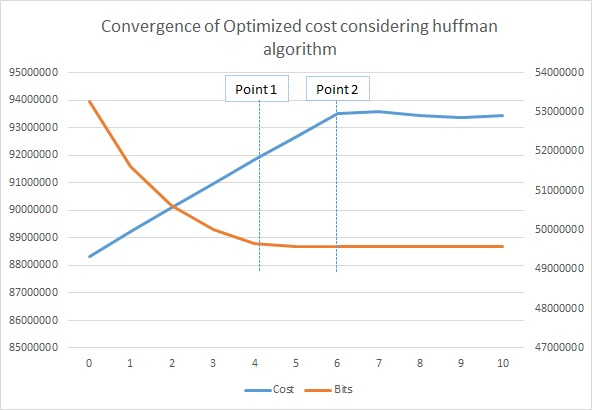
\includegraphics{Images/Drawing4.jpg}
\caption{Convergence of Optimized cost considering Huffman algorithm}
\end{center}
\label{Fig5}
\end{figure}
\section{Conclusion}
\label{sec5}
In this paper we have proposed a new approach for efficient data compression using Huffman code and optimised strategy. The new approach is divided into phases, firstly a cost considering Huffman algorithm are proposed which reduce the cost of the generated codes, these codes are secondary passed by the optimisation algorithm to reduce the global number of bits using a cost penalty.\\
The proposed approach is tested with biological genomic sequence and a performance comparison is made with the standard Huffman code and the cost considering without optimisation. Simulation results showed that the proposed approach is more robust and efficient compared to other competing algorithms because its penalty based optimisation strategy to search the best allocation of codes to different frequencies.

%% The Appendices part is started with the command \appendix;
%% appendix sections are then done as normal sections
%% \appendix

%% \section{}
%% \label{}

%% If you have bibdatabase file and want bibtex to generate the
%% bibitems, please use
%%
%%  \bibliographystyle{elsarticle-num} 
%%  \bibliography{<your bibdatabase>}

%% else use the following coding to input the bibitems directly in the
%% TeX file.

%\begin{thebibliography}{00}

%% \bibitem{label}
%% Text of bibliographic item

%\bibitem{}

%\end{thebibliography}
\section*{References}
\bibliography{mybibfile}
\end{document}
\endinput
%%
%% End of file `elsarticle-template-num.tex'.
